\documentclass{ximera}
\graphicspath{
{./}
{volumes/}
{arclengths/}
{centroids/}
{techniques/}
{applications/}
{series/}
{powerseries/}
{odes/}
{lessons/}
}
\usepackage{booktabs}

\newcommand{\bigmath}[1]{$\displaystyle #1$}
\newcommand{\choicebreak}{}
\newenvironment{type}{}{}
\newenvironment{notes}{}{}
\newenvironment{keywords}{}{}
\newcommand{\offline}{}
\newenvironment{comments}{\begin{feedback}}{\end{feedback}}
\newenvironment{multiplechoice}{\begin{multipleChoice}}{\end{multipleChoice}}
\title{Trigonometric Substitions}
%%%%%\author{Philip T. Gressman}

\begin{document}
\begin{abstract}
  We practice executing trigonometric substitutions.
\end{abstract}
\maketitle

\section*{(Video) Calculus: Single Variable}
\youtube{D_2N1OLQjyk}

\section*{Online Texts}
\begin{itemize}
\item \link[OpenStax II 3.3: Trigonometric Substitution]{https://openstax.org/books/calculus-volume-2/pages/3-3-trigonometric-substitution}
\item \link[Ximera OSU: Trigonometric Substitution]{https://ximera.osu.edu/mooculus/calculus2/trigonometricSubstitution/titlePage}
\item \link[Community Calculus 8.3: Trigonometric Substitution]{https://www.whitman.edu/mathematics/calculus_online/section08.03.html}
\end{itemize}


\section*{Examples}

\begin{example}
(c.f.~Calculus Example 6.4.1) Compute the indefinite integral
\[ \int \sqrt{9 - x^2} dx. \]
\begin{itemize}
\item The structure of this integrand is adapted to a trigonometric substitution of \wordChoice{\choice{secant}\choice[correct]{sine}\choice{tangent}} type, so we let $x = 3 \answer{\sin \theta}$ (to type out the word theta). This gives $dx = 3 \answer{\cos \theta}~d \theta$.
\item Using the identity $\cos^2 \theta + \sin^2 \theta = 1$, the expression $9 - x^2$ can be rewritten using the formula above as $\answer{(3 \cos \theta)^2}$. Therefore
\[ \int \sqrt{9-x^2} dx = \int \answer{9 (\cos \theta)^2} d \theta. \]
\item We use the power reduction formula $\cos^2 t = (1 + \cos 2t)/2$ and conclude
\[ \int \sqrt{9-x^2} dx = \frac{9}{2} \int \left( 1 + \cos 2 \theta \right) d \theta = \frac{9}{2} \left[ \theta + \frac{1}{2} \sin 2 \theta \right] + C. \]
\item Now we construct a reference triangle which is compatible with the substitution we made. In this case, this means we need a right triangle for which $x/3 = \sin \theta$:
\begin{center}
\begin{image}
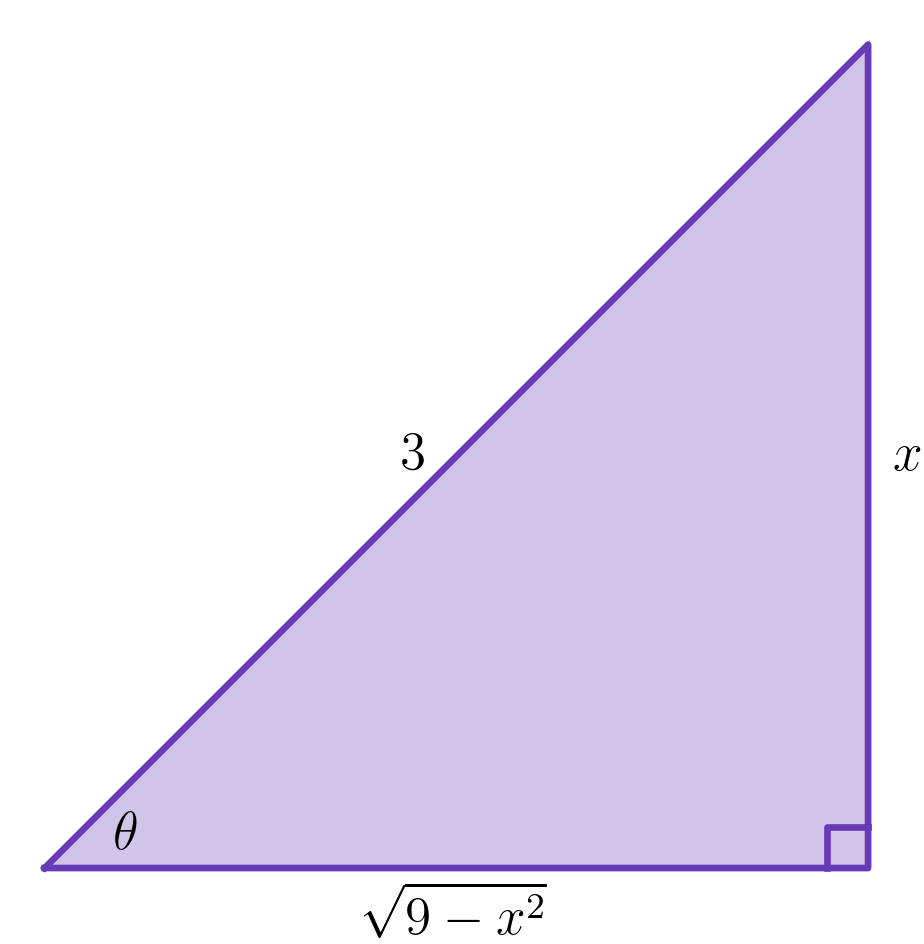
\includegraphics[width=4in]{images/trigsub01.png}
\end{image}
\end{center}

\end{itemize}
\end{example}

\begin{example}

\end{example}


\end{document}
